\chapter{Experimental Design}
\label{ch:experimental_design}

RE-TabSyn is evaluated on six financial benchmark datasets against four baselines across three evaluation pillars: statistical fidelity, machine learning utility, and empirical privacy. All experiments run three random seeds (42, 123, 456); results are reported as mean $\pm$ standard deviation.

\section{Benchmark Datasets}

Table~\ref{tab:datasets} summarises the six financial benchmark datasets. Each covers a distinct financial domain and a different imbalance severity, testing the method under both extreme and moderate imbalance.

\renewcommand{\arraystretch}{1.2}

\begin{xltabular}{\textwidth}{|X|c|c|c|c|X|}
\caption{Benchmark dataset characteristics}
\label{tab:datasets} \\

\noalign{\hrule height\arrayrulewidth}
\textbf{Dataset} & \textbf{Samples} & \textbf{Num.} & \textbf{Cat.} & \textbf{Min. \%} & \textbf{Domain} \\
\hline
\noalign{\vskip 4pt}
\hline
\endfirsthead

\noalign{\hrule height\arrayrulewidth}
\textbf{Dataset} & \textbf{Samples} & \textbf{Num.} & \textbf{Cat.} & \textbf{Min. \%} & \textbf{Domain} \\
\hline
\noalign{\vskip 4pt}
\hline
\endhead

\hline
\multicolumn{6}{r}{\small\itshape Continued on next page} \\
\endfoot

\hline
\endlastfoot

Adult Income & 45,222 & 6 & 8 & 24.8\% & Income prediction \\
\hline
German Credit & 1,000 & 7 & 13 & 30.0\% & Credit risk \\
\hline
Bank Marketing & 41,188 & 10 & 10 & 11.3\% & Marketing response \\
\hline
Credit Approval & 690 & 6 & 9 & 44.5\% & Credit scoring \\
\hline
Lending Club & 10,000 & 8 & 4 & 20.0\% & Loan default \\
\hline
Polish Bankruptcy & 5,000 & 64 & 0 & 4.8\% & Corporate bankruptcy \\
\hline

\end{xltabular}

Table~\ref{tab:dataset_sources} provides the source and provenance for each dataset.

\renewcommand{\arraystretch}{1.2}

\begin{xltabular}{\textwidth}{|c|X|X|X|}
\caption{Dataset sources and provenance}
\label{tab:dataset_sources} \\

\noalign{\hrule height\arrayrulewidth}
\textbf{Dataset} & \textbf{Repository} & \textbf{URL} & \textbf{Original Source / Creators} \\
\hline
\noalign{\vskip 4pt}
\hline
\endfirsthead

\noalign{\hrule height\arrayrulewidth}
\textbf{Dataset} & \textbf{Repository} & \textbf{URL} & \textbf{Original Source / Creators} \\
\hline
\noalign{\vskip 4pt}
\hline
\endhead

\hline
\multicolumn{4}{r}{\small\itshape Continued on next page} \\
\endfoot

\hline
\endlastfoot

Adult Income & UCI ML Repository & \url{https://archive.ics.uci.edu/dataset/2/adult} & Kohavi \& Becker (1996), U.S. Census Bureau \\
\hline
German Credit & UCI ML Repository & \url{https://archive.ics.uci.edu/dataset/144/statlog+german+credit+data} & Prof.\ H. Hofmann, Universit\"{a}t Hamburg (1994) \\
\hline
Bank Marketing & UCI ML Repository & \url{https://archive.ics.uci.edu/dataset/222/bank+marketing} & Moro, Cortez \& Rita (2014), Portuguese bank records \\
\hline
Credit Approval & UCI ML Repository & \url{https://archive.ics.uci.edu/dataset/27/credit+approval} & J.R.\ Quinlan (1987), anonymised for privacy \\
\hline
Lending Club & Kaggle / LendingClub Corp. & \url{https://www.kaggle.com/datasets/wordsforthewise/lending-club} & LendingClub Corporation (SEC-regulated, publicly traded) \\
\hline
Polish Bankruptcy & UCI ML Repository & \url{https://archive.ics.uci.edu/dataset/365/polish+companies+bankruptcy+data} & Zieba et al.\ (2016), EMIS financial database \\
\hline

\end{xltabular}

Adult Income \cite{uci_adult}: US Census data on 45,222 individuals with features including age, education level, occupation, and weekly working hours. The label indicates whether annual income exceeds \$50{,}000. The largest dataset in the benchmark, it tests whether RE-TabSyn scales to real-world sizes without degradation.

German Credit \cite{uci_german}: 1,000 loan applicants from a German bank, classified as good or bad credit risks. With 13 categorical and only 7 numerical features, it is the most categorically dense dataset in the benchmark.

Bank Marketing \cite{uci_bankmarketing}: 41,188 direct marketing calls by a Portuguese bank between 2008 and 2013. The label indicates whether the client subscribed to a term deposit.

Credit Approval \cite{uci_creditapproval}: 690 anonymised credit applications from J.R.\ Quinlan's 1987 study. At 44.5\% minority, it is nearly balanced, testing that RE-TabSyn does not over-correct when minority boosting is not needed.

Lending Club \cite{kaggle_lendingclub}: Application attributes and repayment outcomes for a stratified 10,000-record subsample of LendingClub Corporation loans. The label is loan default (minority, 20\%).

Polish Bankruptcy \cite{uci_polishbankruptcy}: Financial ratio data for Polish companies from the EMIS database, covering 2000--2012. Contains 64 purely numerical financial ratios with a 4.8\% bankruptcy rate --- the most extreme imbalance and the highest dimensionality in the benchmark.

\section{Model Configurations}

Table~\ref{tab:hyperparams} lists all RE-TabSyn hyperparameters.

\renewcommand{\arraystretch}{1.2}

\begin{xltabular}{\textwidth}{|X|X|X|}
\caption{RE-TabSyn hyperparameter reference}
\label{tab:hyperparams} \\

\noalign{\hrule height\arrayrulewidth}
\textbf{Component} & \textbf{Hyperparameter} & \textbf{Value} \\
\hline
\noalign{\vskip 4pt}
\hline
\endfirsthead

\noalign{\hrule height\arrayrulewidth}
\textbf{Component} & \textbf{Hyperparameter} & \textbf{Value} \\
\hline
\noalign{\vskip 4pt}
\hline
\endhead

\hline
\multicolumn{3}{r}{\small\itshape Continued on next page} \\
\endfoot

\hline
\endlastfoot

\textbf{VAE} & Encoder hidden dims & [256, 128] \\
\hline
 & Decoder hidden dims & [128, 256] \\
\hline
 & Latent dimension $d$ & 64 \\
\hline
 & Activation & ReLU \\
\hline
 & KL weight $\beta$ & 0.1 \\
\hline

\textbf{Diffusion (DiT)} & Number of layers & 4 \\
\hline
 & Hidden dimension & 256 \\
\hline
 & Attention heads & 4 \\
\hline
 & Head dimension & 64 \\
\hline
 & Timesteps $T$ & 1000 \\
\hline
 & Noise schedule & Linear \\
\hline
 & $\beta_1$ (start) & $10^{-4}$ \\
\hline
 & $\beta_T$ (end) & 0.02 \\
\hline

\textbf{Embeddings} & Time embed dim & 128 \\
\hline
 & Time projection dim & 256 \\
\hline
 & Class vocab size & 3 (0, 1, $\emptyset$) \\
\hline
 & Class embed dim & 256 \\
\hline

\textbf{CFG} & Label dropout $p_{uncond}$ & 0.10 \\
\hline
 & Guidance scale $w$ & 2.0 \\
\hline

\textbf{Training} & Optimiser & Adam \\
\hline
 & Learning rate & $10^{-3}$ \\
\hline
 & Batch size & 256 \\
\hline
 & Epochs per phase & 100 \\
\hline

\textbf{Evaluation} & Train/test split & 80\% / 20\% \\
\hline
 & Random seeds & 42, 123, 456 \\
\hline

\end{xltabular}

\subsection{RE-TabSyn architecture}

VAE Encoder: MLP with hidden dimensions [256, 128] and ReLU activations. Output: mean vector $\mu \in \mathbb{R}^{64}$ and log-variance vector $\log \sigma^2 \in \mathbb{R}^{64}$.

VAE Decoder: Mirror architecture [128, 256] with separate output heads --- a linear projection for numerical features and a per-column softmax projection for categorical features.

Diffusion Backbone (DiT): Diffusion Transformer with 4 layers, hidden dimension 256, 4 attention heads. Noise schedule: $T = 1000$ timesteps, linear $\beta$ from $\beta_1 = 10^{-4}$ to $\beta_T = 0.02$.

Guidance: Label dropout $p_{uncond} = 0.10$ during training; guidance scale $w = 2.0$ during inference.

Embeddings: Sinusoidal time embeddings projected to 256 dimensions via a two-layer MLP. Learned class embeddings for 3 tokens (class 0, class 1, null $\emptyset$).

\subsection{Baseline configurations}

All baselines use their official codebases:

CTGAN \cite{xu2019ctgan}: Mode-specific normalization, PAC discriminator (pack size 10), embedding dimension 128, generator and discriminator hidden dimensions [256, 256], batch size 500, 100 epochs. Implemented via the SDV library.

TVAE: Same tabular preprocessing as CTGAN, embedding dimension 128, encoder and decoder hidden dimensions [128, 128], 100 epochs. Implemented via SDV.

TabDDPM \cite{kotelnikov2023tabddpm}: Gaussian diffusion for numerical features, multinomial diffusion for categorical features, MLP backbone [256, 256, 256], 1,000 diffusion steps, 100 epochs.

TabSyn \cite{zhang2024tabsyn}: VAE with Transformer-based latent diffusion, no CFG. Each feature is tokenized separately before encoding. The highest-fidelity tabular synthesis baseline at the time of this work.

\subsection{Method comparison at a glance}

Table~\ref{tab:method_comparison} summarises the architectural properties of all five methods.

\renewcommand{\arraystretch}{1.2}

\begin{xltabular}{\textwidth}{|X|X|X|X|X|X|}
\caption{Architectural comparison across methods}
\label{tab:method_comparison} \\

\noalign{\hrule height\arrayrulewidth}
\textbf{Property} & \textbf{CTGAN} & \textbf{TVAE} & \textbf{TabDDPM} & \textbf{TabSyn} & \textbf{RE-TabSyn} \\
\hline
\noalign{\vskip 4pt}
\hline
\endfirsthead

\noalign{\hrule height\arrayrulewidth}
\textbf{Property} & \textbf{CTGAN} & \textbf{TVAE} & \textbf{TabDDPM} & \textbf{TabSyn} & \textbf{RE-TabSyn} \\
\hline
\noalign{\vskip 4pt}
\hline
\endhead

\hline
\multicolumn{6}{r}{\small\itshape Continued on next page} \\
\endfoot

\hline
\endlastfoot

Framework & GAN & VAE & Diffusion & VAE + Diffusion & VAE + Diffusion + CFG \\
\hline
Generative model & Generator & Decoder & MLP diffusion & DiT diffusion & DiT diffusion \\
\hline
Latent space & No & Yes (128-d) & No & Yes (learned) & Yes (64-d Gaussian) \\
\hline
Handles mixed types & Yes (mode norm.) & Yes (mode norm.) & Poor & Yes & Yes \\
\hline
Minority class control & No & No & No & No & Yes (CFG, $w$) \\
\hline
Class conditioning & No & No & No & No & Yes \\
\hline
Training phases & 1 & 1 & 1 & 2 & 2 \\
\hline
Fast sampling possible & N/A & N/A & DDIM & DDIM & DDIM \\
\hline
Formal DP support & No & No & No & No & Planned (Opacus) \\
\hline

\end{xltabular}

RE-TabSyn is the only method among the five that offers minority class control. Every other method generates data that mirrors the training class distribution at inference time.

\section{Training Procedures}

Training proceeds in two sequential phases that decouple representation learning from generative modeling. Figure~\ref{fig:two_phase_training} shows the structure.

\begin{figure}[H]
\centering
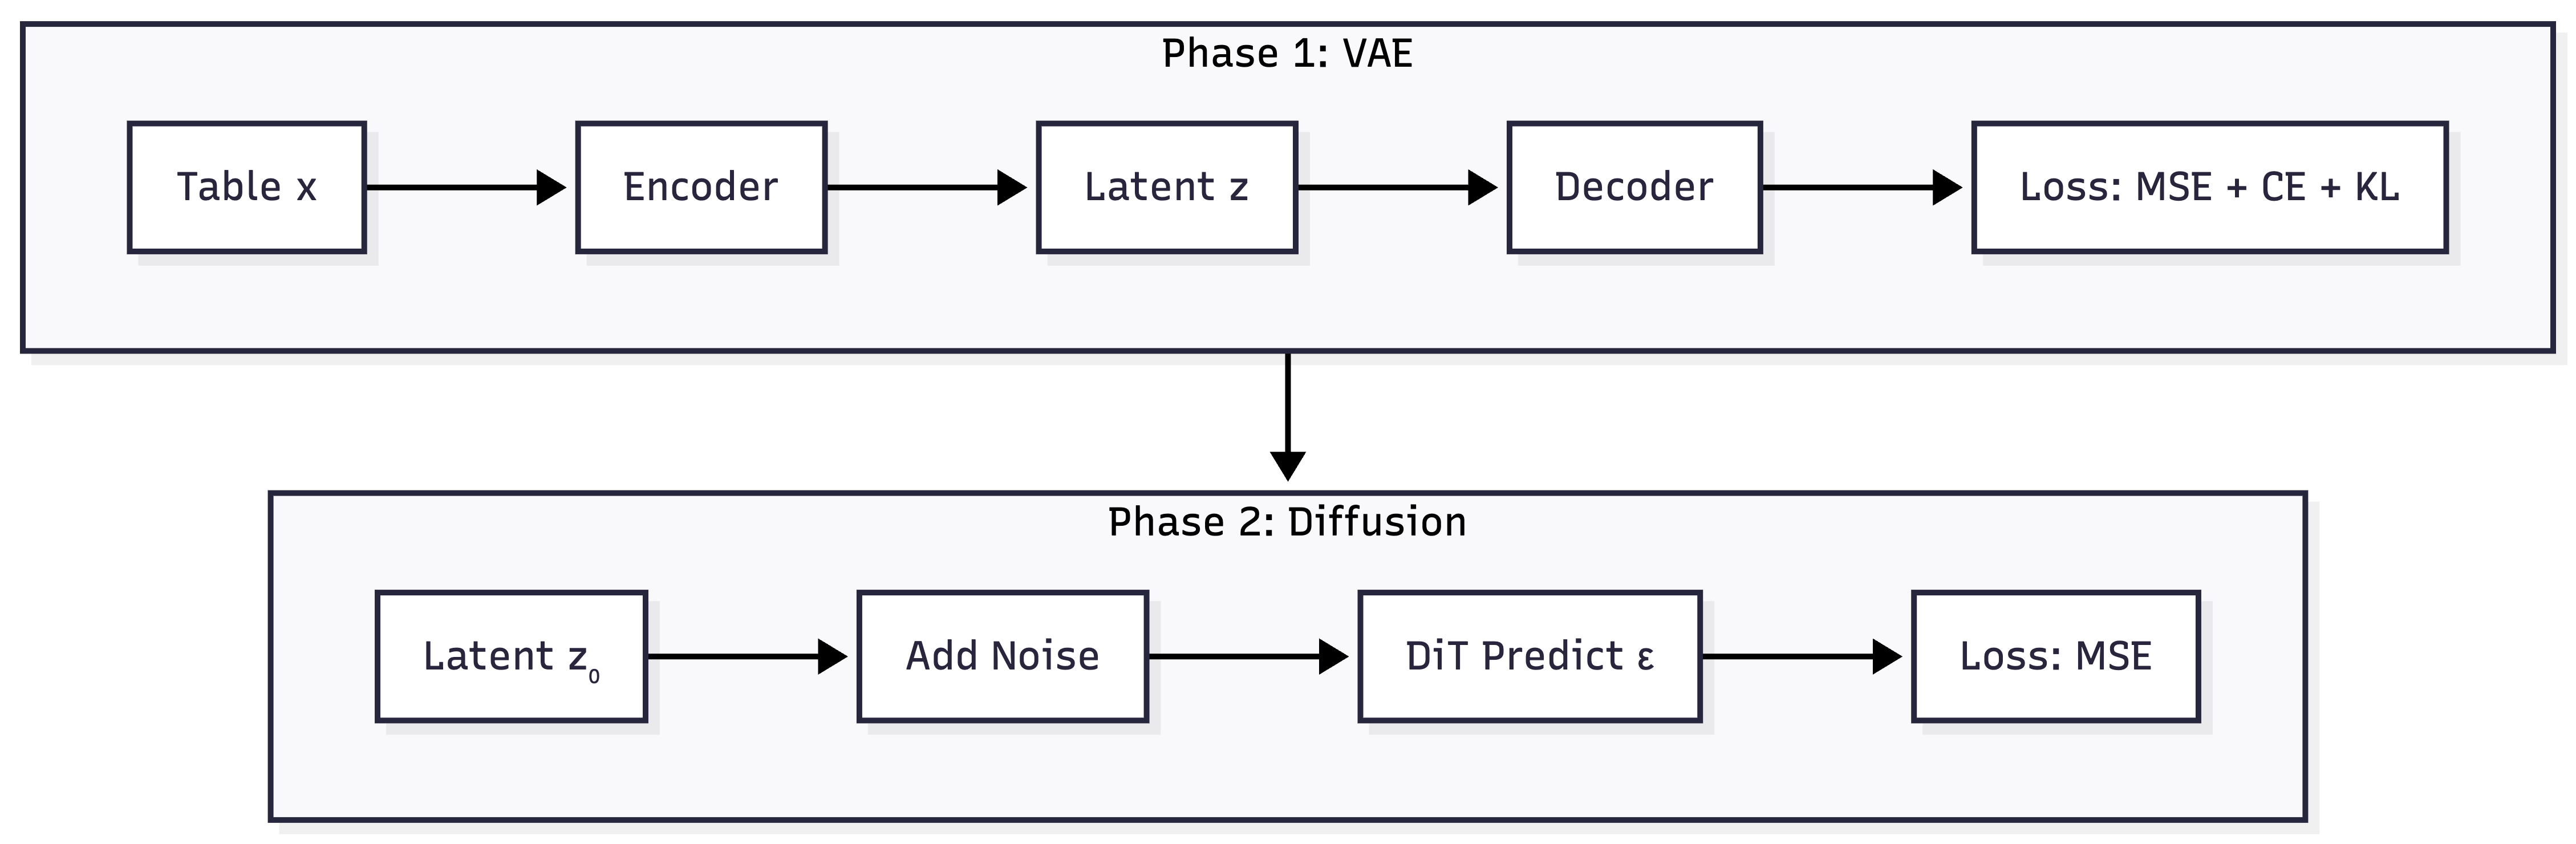
\includegraphics[width=\textwidth]{img/two_phase_training.png}
\caption{Two-phase VAE and diffusion training.}
\label{fig:two_phase_training}
\end{figure}

\textbf{Phase 1 --- VAE Training (Epochs 1--100):}

\begin{enumerate}
    \item Data is preprocessed and split 80/20 into training and test sets. The test set is held out entirely during training.

    \item The VAE minimizes $\mathcal{L}_{VAE} = \mathcal{L}_{MSE} + \mathcal{L}_{CE} + 0.1 \cdot \mathcal{L}_{KL}$ on the training set.

    \item KL weight $\beta = 0.1$ is fixed (not annealed), achieving stable training without posterior collapse across all six datasets.

    \item Adam optimizer, learning rate $10^{-3}$, batch size 256.

    \item Training converges within 50--80 epochs; the checkpoint with lowest validation loss is used for latent encoding.
\end{enumerate}

\begin{figure}[H]
\centering
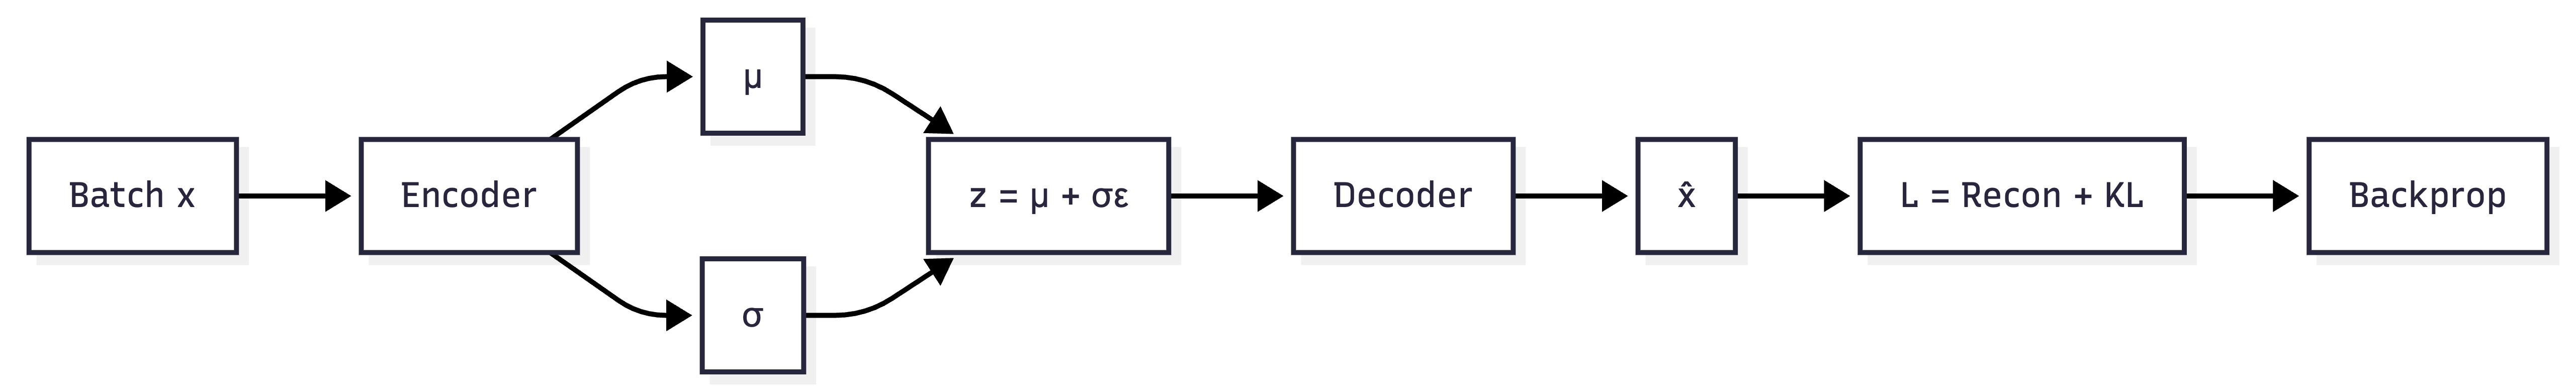
\includegraphics[width=\textwidth]{img/vae_training_loop.png}
\caption{VAE training loop: encode, sample, decode.}
\label{fig:vae_training_loop}
\end{figure}

\textbf{Phase 2 --- Diffusion Training (Epochs 1--100):}

\begin{enumerate}
    \item VAE weights are frozen. This ensures the latent space geometry does not shift during Phase 2, which would invalidate the already-learned diffusion parameters.

    \item All training data is encoded to 64-dimensional latents once using the frozen encoder. The resulting vectors are cached to avoid re-encoding at every training step.

    \item Each training step: sample timestep $t \sim \mathcal{U}(1, 1000)$ and noise $\boldsymbol{\epsilon} \sim \mathcal{N}(\mathbf{0}, \mathbf{I})$; apply label dropout ($p = 0.10$); compute $\mathbf{z}_t$; predict noise with DiT; backpropagate MSE loss.

    \item Same Adam optimizer and batch size as Phase 1.

    \item All experiments run with three random seeds (42, 123, 456) to assess result variance.
\end{enumerate}

\begin{figure}[H]
\centering
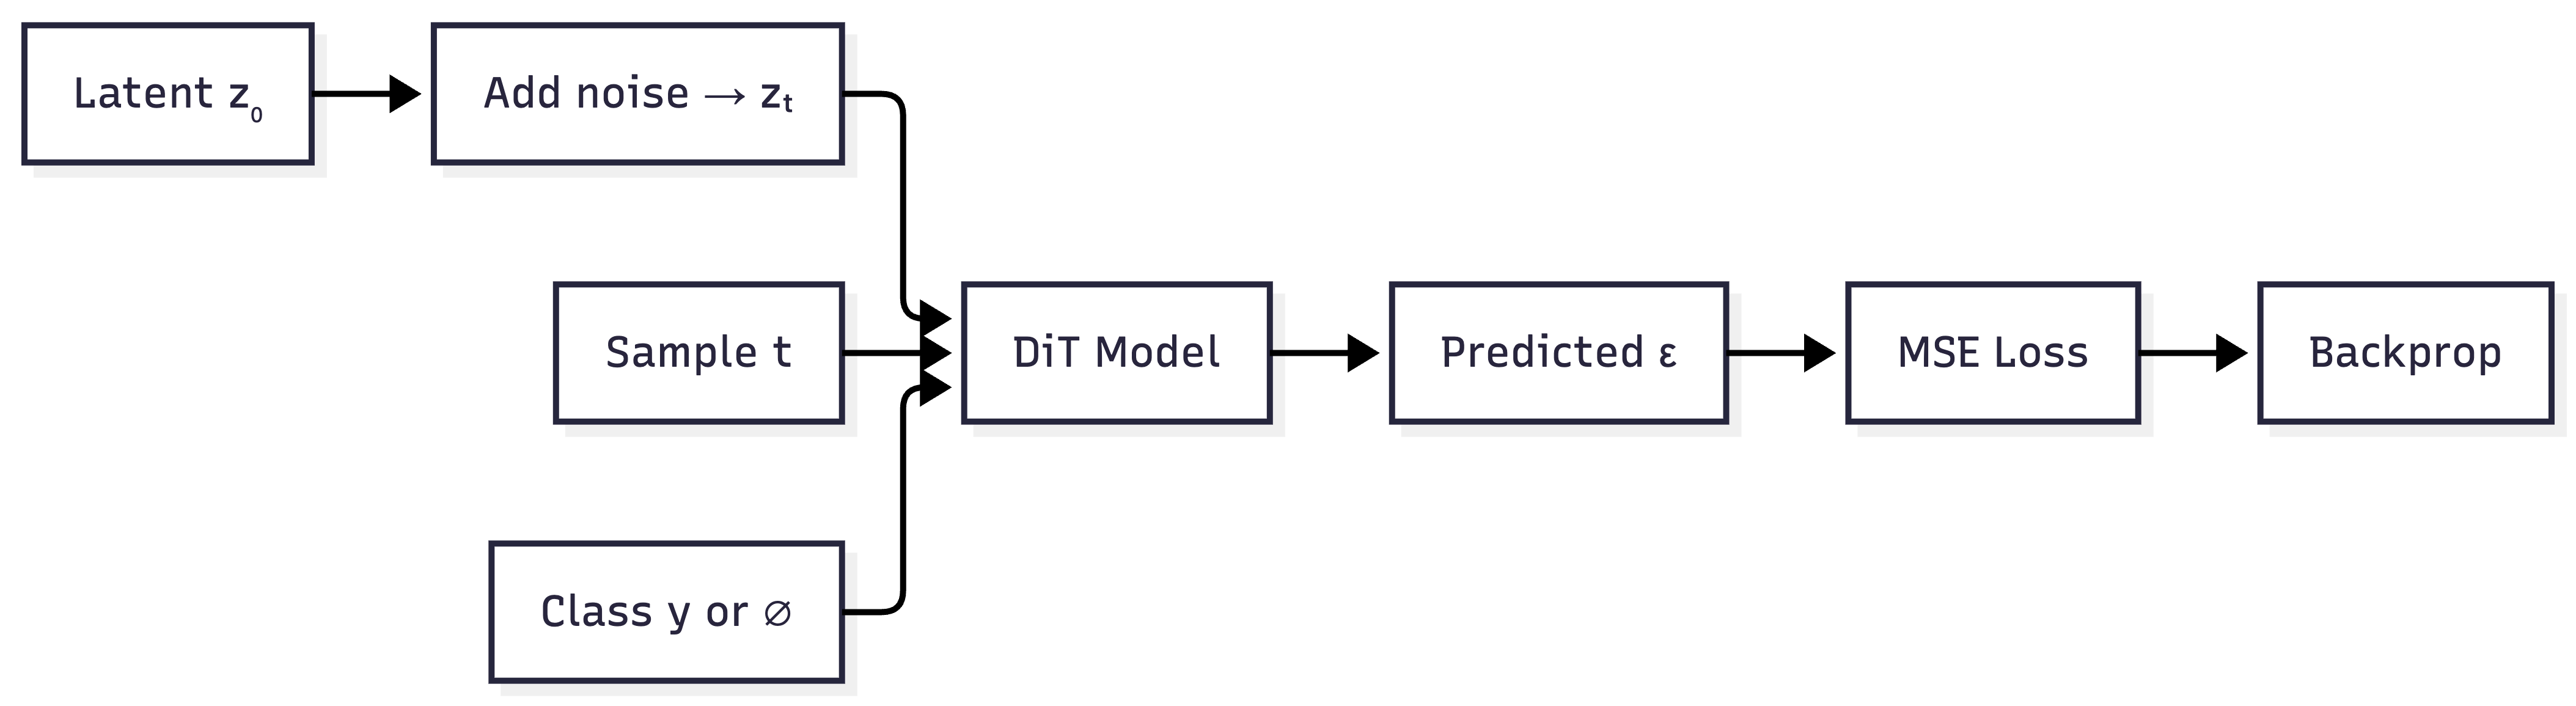
\includegraphics[width=\textwidth]{img/diffusion_training_loop.png}
\caption{Diffusion training loop on frozen latents.}
\label{fig:diffusion_training_loop}
\end{figure}

\section{Evaluation Framework}

The evaluation follows a three-pillar framework. Figure~\ref{fig:evaluation_framework} shows the structure.

\begin{figure}[H]
\centering
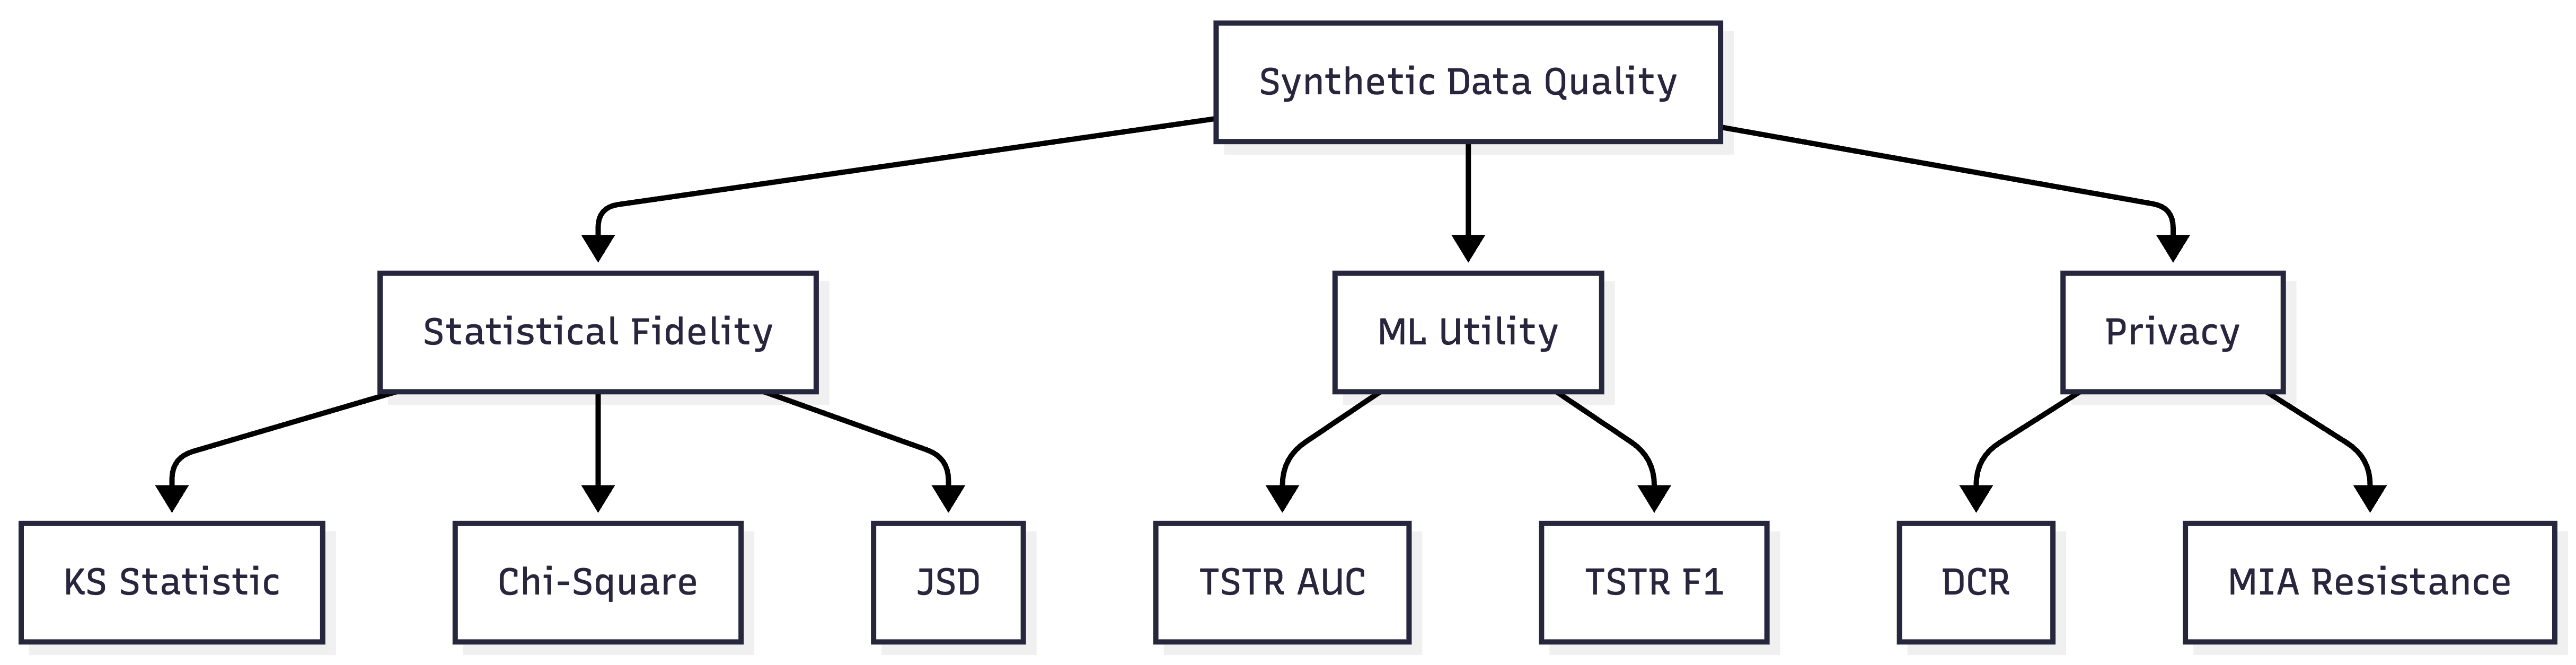
\includegraphics[width=\textwidth]{img/evaluation_framework.png}
\caption{Three-pillar evaluation framework.}
\label{fig:evaluation_framework}
\end{figure}

\subsection{Pillar 1: Statistical fidelity}

Kolmogorov-Smirnov (KS) Statistic \cite{massey1951ks}: For each numerical column, the maximum absolute difference between the empirical CDFs of real and synthetic data:
\[
D_{KS} = \sup_x |F_{real}(x) - F_{synth}(x)|
\]
Values range from 0 (identical distributions) to 1 (completely different). The average KS across all numerical columns is reported. The KS test is non-parametric: it detects differences anywhere in the distribution, not just in the mean or variance.

Correlation Preservation: Mean absolute difference between the pairwise Pearson correlation matrices of real and synthetic data:
\[
\text{Corr Error} = \frac{1}{d^2} \sum_{i,j} |r_{ij}^{real} - r_{ij}^{synth}|
\]
This captures joint distribution quality that the KS statistic misses: two datasets could have identical marginal distributions while having entirely wrong correlation structures.

\subsection{Pillar 2: Machine learning utility}

Low KS does not guarantee a model trained on synthetic data will perform well on real data. The TSTR protocol tests this directly: train on synthetic, test on real, measure the gap.

\begin{figure}[H]
\centering
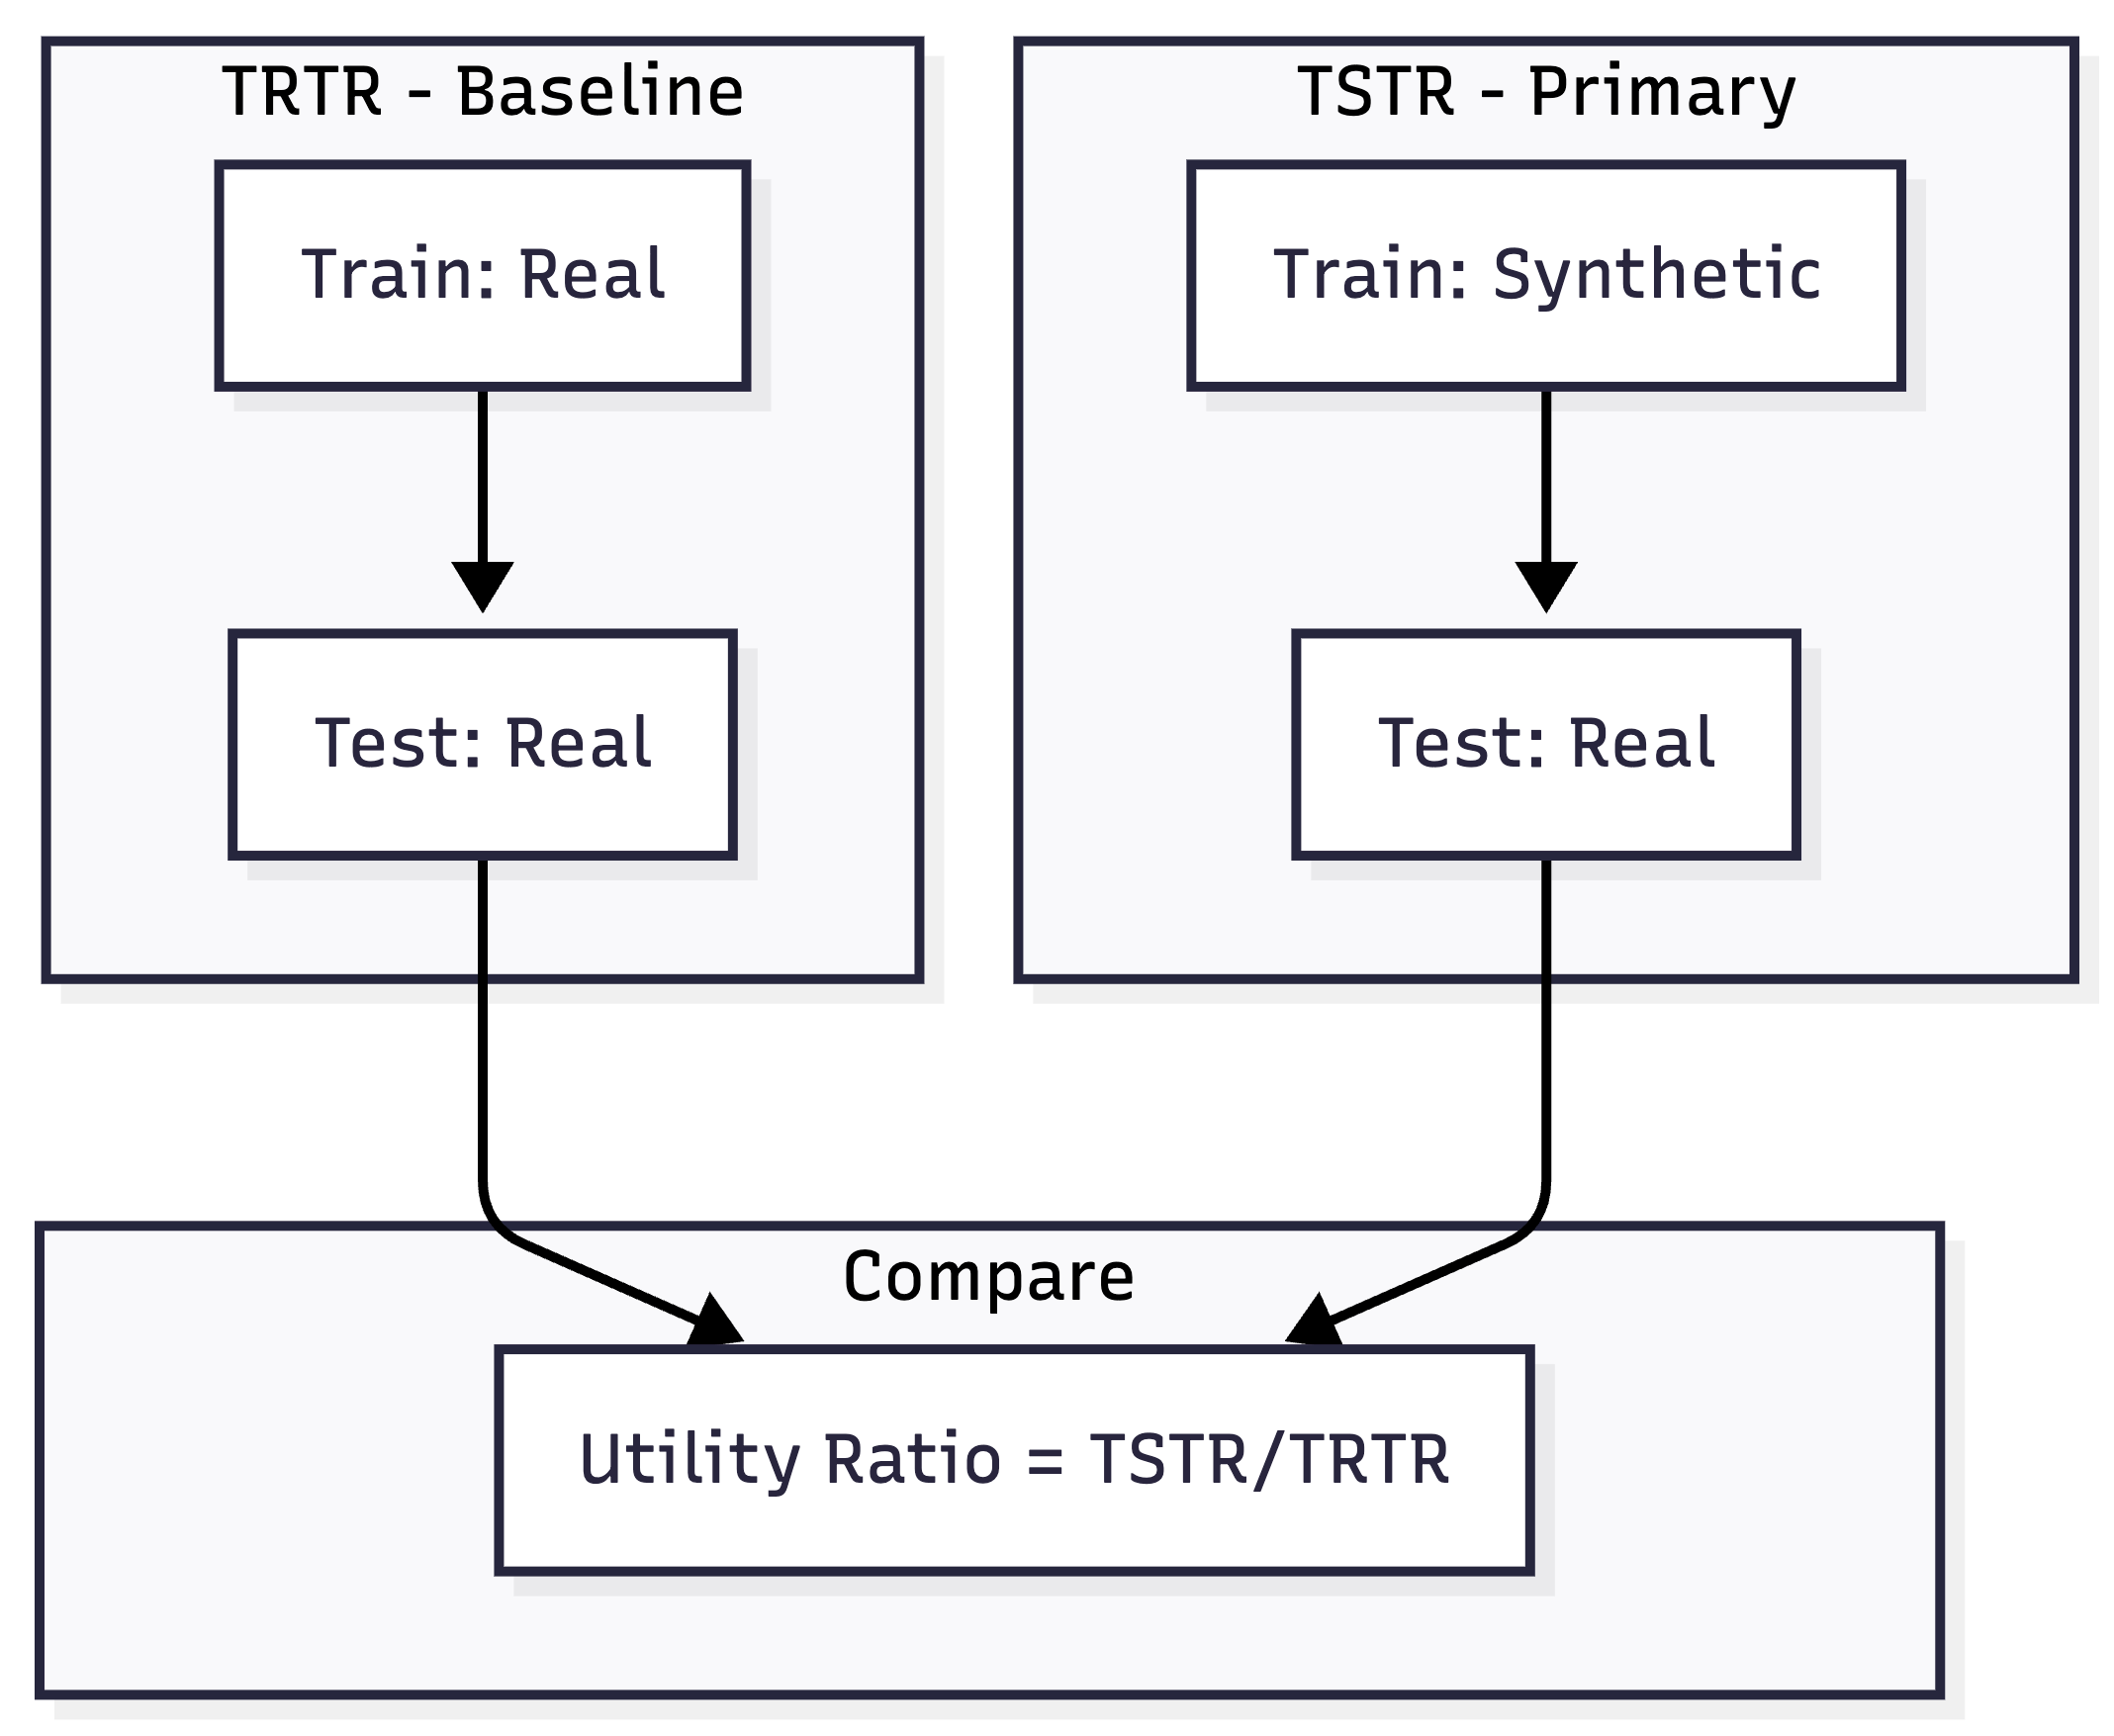
\includegraphics[width=0.45\textwidth]{img/tstr_trtr.png}
\caption{TSTR vs.\ TRTR utility ratio.}
\label{fig:tstr_trtr}
\end{figure}

TSTR AUC-ROC: An XGBoost \cite{chen2016xgboost} classifier is trained exclusively on synthetic data and evaluated on the real held-out test set. XGBoost hyperparameters are fixed across all experiments (learning rate 0.1, 100 estimators, max depth 6) so performance differences reflect synthetic data quality, not classifier tuning.

Minority F1-Score: The F1-score for the minority class under the TSTR protocol:

\[
F1_{minority} = \frac{2 \cdot \text{Precision}_{minority} \cdot \text{Recall}_{minority}}{\text{Precision}_{minority} + \text{Recall}_{minority}}
\]

This is the primary utility metric for imbalanced tasks. Overall AUC can be misleading for highly imbalanced datasets; F1 measures whether the model actually catches minority events.

\subsection{Pillar 3: Privacy preservation}

DCR measures the distance from each synthetic sample to its nearest real training record. A very low DCR on any sample is a sign the model may have memorised that record rather than learned from it.

\begin{figure}[H]
\centering
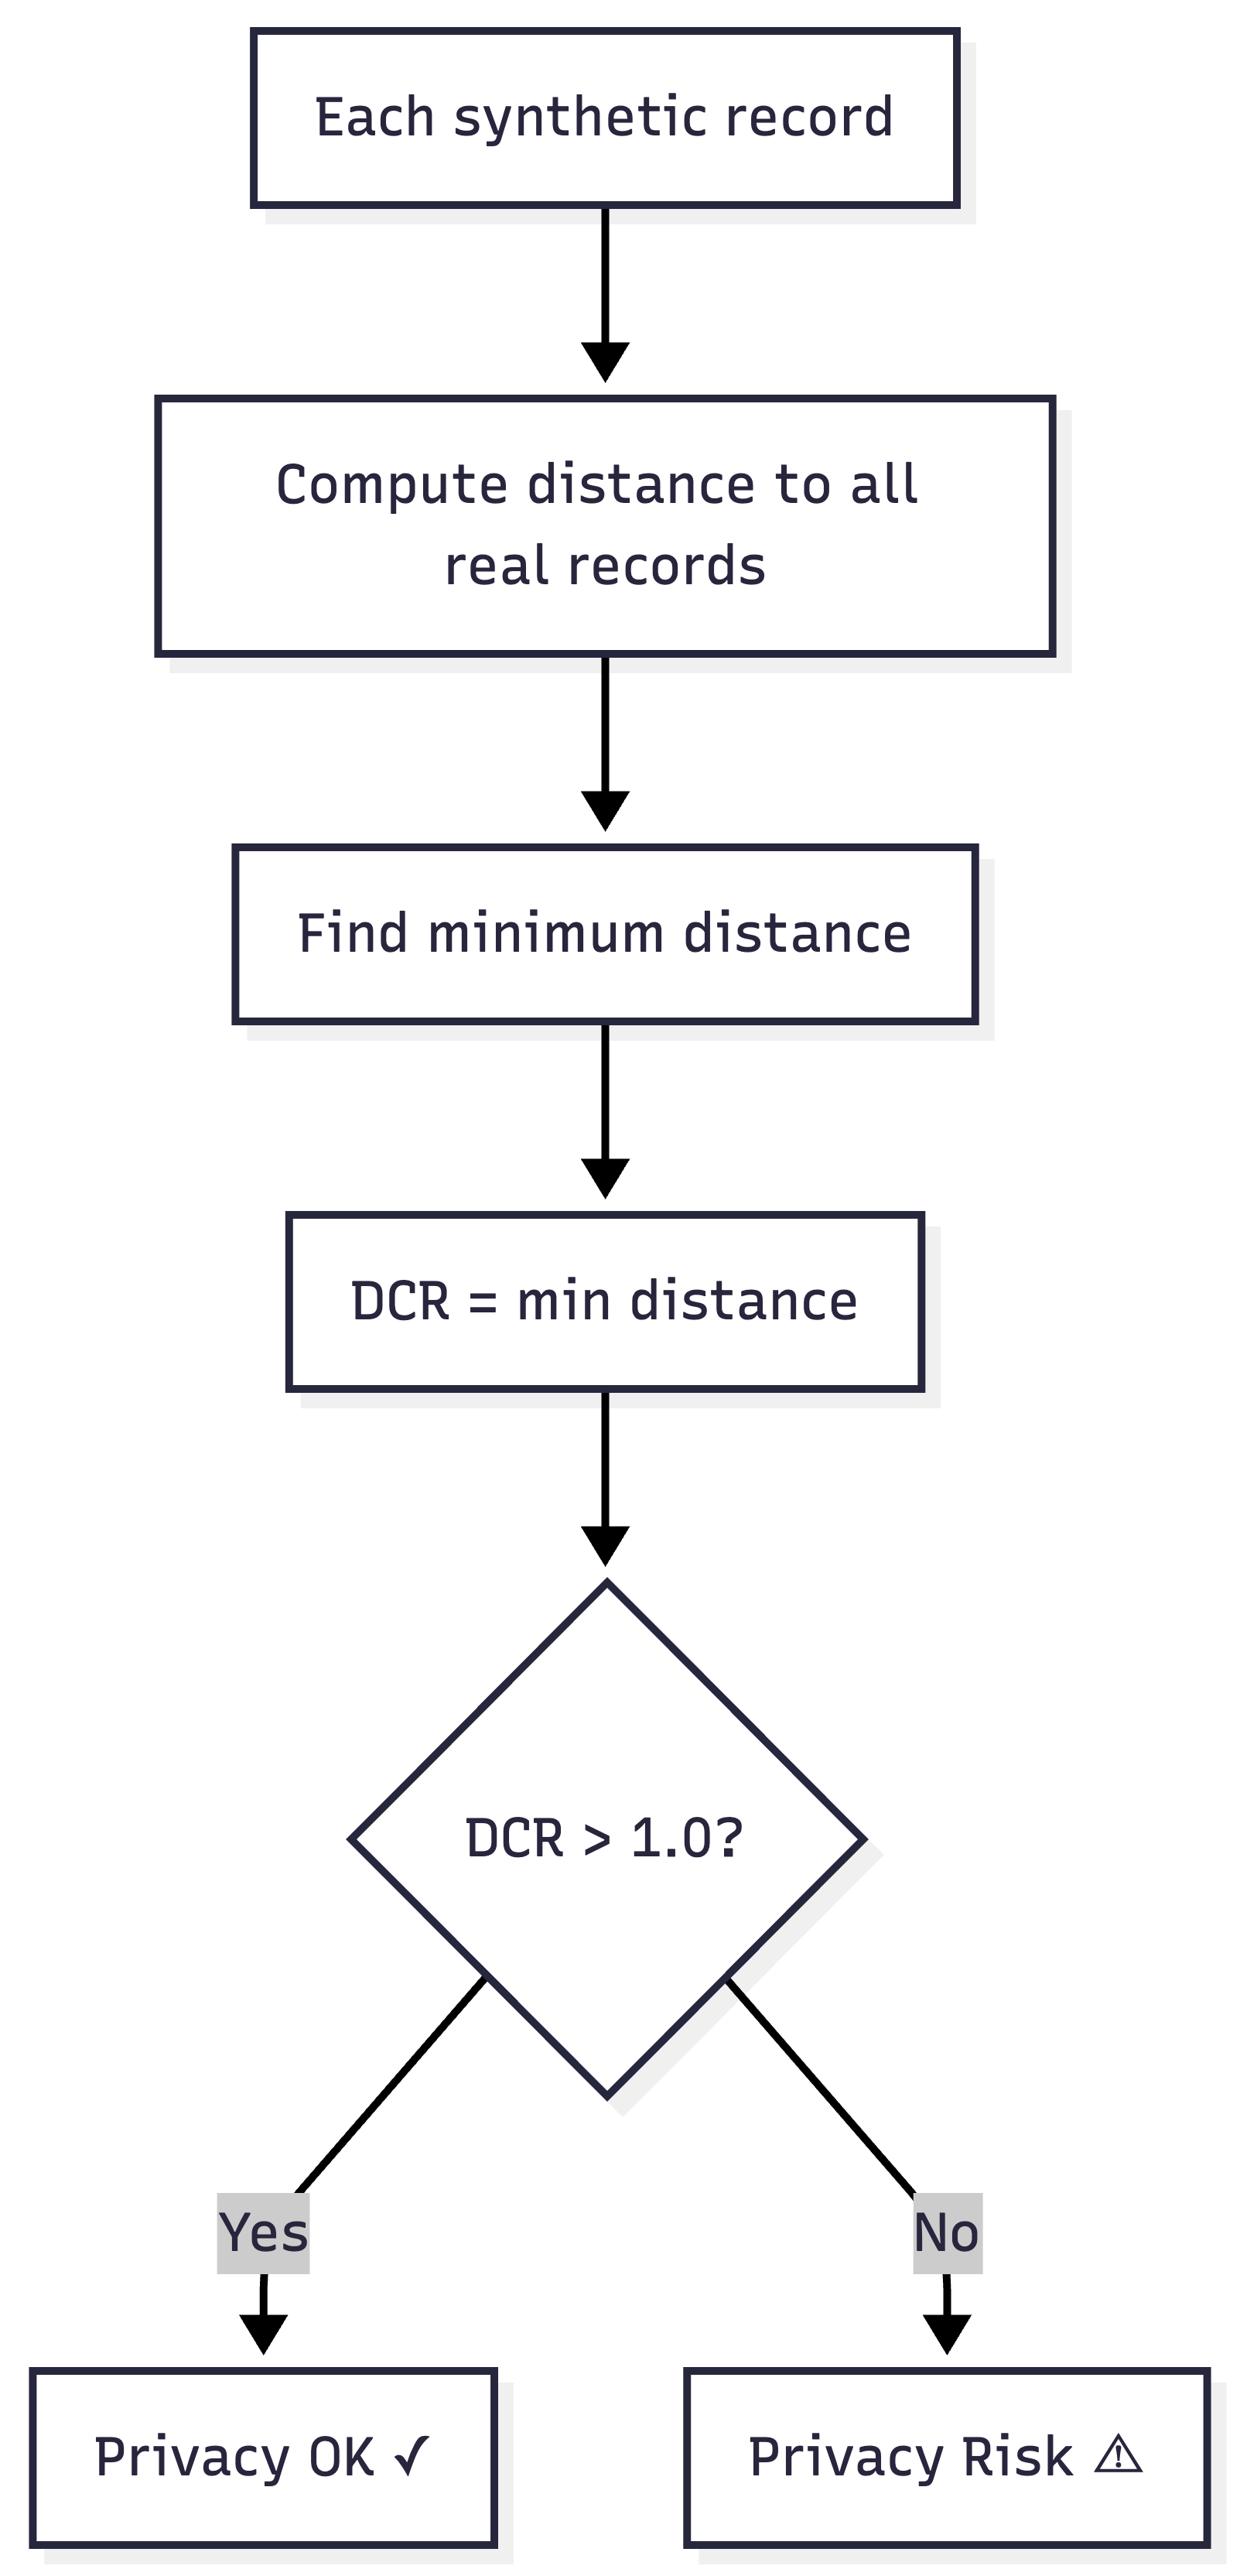
\includegraphics[width=0.33\textwidth]{img/dcr_flowchart.png}
\caption{DCR computation and privacy threshold.}
\label{fig:dcr_flowchart}
\end{figure}

Distance to Closest Record (DCR): For each synthetic sample $\tilde{\mathbf{x}}_i$, the Euclidean distance to the nearest real training sample:
\[
\text{DCR}(\tilde{\mathbf{x}}_i) = \min_{j} \|\tilde{\mathbf{x}}_i - \mathbf{x}_j\|_2
\]
Mean DCR measures average privacy across all synthetic samples. Minimum DCR identifies the worst-case record. Higher values indicate better empirical privacy. All metrics are computed independently for each of the three random seeds.
